\documentclass{standalone}
\usepackage{tikz}
\usetikzlibrary{patterns, positioning}

\begin{document}
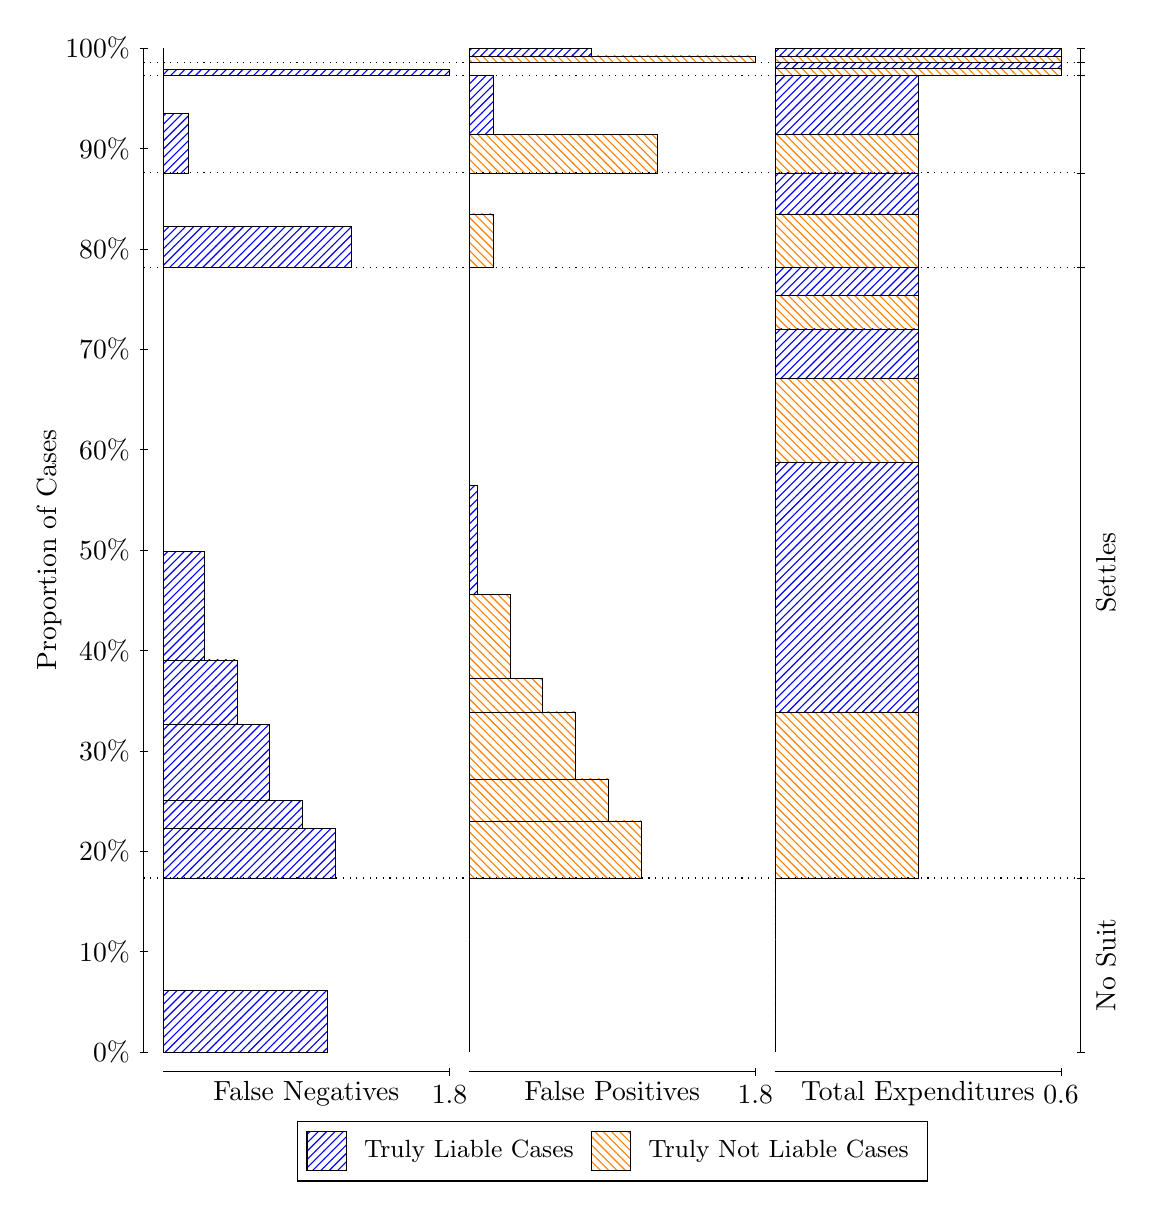
\begin{tikzpicture}
\draw[black, very thin] (1.5,1.75) -- (1.5,14.5);
\node[rotate=90, anchor=center] at (0.3, 8.125) {Proportion of Cases};
\draw[black, very thin] (1.45,1.75) -- (1.55,1.75);
\node[anchor=east] at (1.45, 1.75) {0\%};
\draw[black, very thin] (1.45,3.025) -- (1.55,3.025);
\node[anchor=east] at (1.45, 3.025) {10\%};
\draw[black, very thin] (1.45,4.3) -- (1.55,4.3);
\node[anchor=east] at (1.45, 4.3) {20\%};
\draw[black, very thin] (1.45,5.575) -- (1.55,5.575);
\node[anchor=east] at (1.45, 5.575) {30\%};
\draw[black, very thin] (1.45,6.85) -- (1.55,6.85);
\node[anchor=east] at (1.45, 6.85) {40\%};
\draw[black, very thin] (1.45,8.125) -- (1.55,8.125);
\node[anchor=east] at (1.45, 8.125) {50\%};
\draw[black, very thin] (1.45,9.4) -- (1.55,9.4);
\node[anchor=east] at (1.45, 9.4) {60\%};
\draw[black, very thin] (1.45,10.675) -- (1.55,10.675);
\node[anchor=east] at (1.45, 10.675) {70\%};
\draw[black, very thin] (1.45,11.95) -- (1.55,11.95);
\node[anchor=east] at (1.45, 11.95) {80\%};
\draw[black, very thin] (1.45,13.225) -- (1.55,13.225);
\node[anchor=east] at (1.45, 13.225) {90\%};
\draw[black, very thin] (1.45,14.5) -- (1.55,14.5);
\node[anchor=east] at (1.45, 14.5) {100\%};

\draw[black, very thin] (13.4,1.75) -- (13.4,14.5);
\draw[black, very thin] (13.35,1.75) -- (13.45,1.75);
\node[anchor=west] at (13.35, 1.75) {};
\draw[black, very thin] (13.35,3.9589) -- (13.45,3.9589);
\node[anchor=west] at (13.35, 3.9589) {};
\draw[black, very thin] (13.35,11.711) -- (13.45,11.711);
\node[anchor=west] at (13.35, 11.711) {};
\draw[black, very thin] (13.35,12.914) -- (13.45,12.914);
\node[anchor=west] at (13.35, 12.914) {};
\draw[black, very thin] (13.35,14.156) -- (13.45,14.156);
\node[anchor=west] at (13.35, 14.156) {};
\draw[black, very thin] (13.35,14.32) -- (13.45,14.32);
\node[anchor=west] at (13.35, 14.32) {};
\draw[black, very thin] (13.35,14.5) -- (13.45,14.5);
\node[anchor=west] at (13.35, 14.5) {};

\draw[black, very thin, pattern color=blue, pattern=north east lines] (1.75,1.75) rectangle (3.8262,2.5285);
\draw[black, very thin, pattern color=orange, pattern=north west lines] (1.75,2.5285) rectangle (1.75,3.9589);
\draw[black, very thin, pattern color=blue, pattern=north east lines] (1.75,3.9589) rectangle (3.93,4.5895);
\draw[black, very thin, pattern color=blue, pattern=north east lines] (1.75,4.5895) rectangle (3.5148,4.9419);
\draw[black, very thin, pattern color=blue, pattern=north east lines] (1.75,4.9419) rectangle (3.0995,5.9092);
\draw[black, very thin, pattern color=blue, pattern=north east lines] (1.75,5.9092) rectangle (2.6843,6.729);
\draw[black, very thin, pattern color=blue, pattern=north east lines] (1.75,6.729) rectangle (2.269,8.1067);
\draw[black, very thin, pattern color=orange, pattern=north west lines] (1.75,8.1067) rectangle (1.75,11.711);
\draw[black, very thin, pattern color=blue, pattern=north east lines] (1.75,11.711) rectangle (4.1376,12.233);
\draw[black, very thin, pattern color=orange, pattern=north west lines] (1.75,12.233) rectangle (1.75,12.914);
\draw[black, very thin, pattern color=blue, pattern=north east lines] (1.75,12.914) rectangle (2.0614,13.666);
\draw[black, very thin, pattern color=orange, pattern=north west lines] (1.75,13.666) rectangle (1.75,14.156);
\draw[black, very thin, pattern color=blue, pattern=north east lines] (1.75,14.156) rectangle (5.3833,14.231);
\draw[black, very thin, pattern color=orange, pattern=north west lines] (1.75,14.231) rectangle (1.75,14.32);
\draw[black, very thin, pattern color=orange, pattern=north west lines] (1.75,14.32) rectangle (1.75,14.401);
\draw[black, very thin, pattern color=blue, pattern=north east lines] (1.75,14.401) rectangle (1.75,14.5);
\draw[black, very thin, pattern color=orange, pattern=north west lines] (5.6333,1.75) rectangle (5.6333,3.1805);
\draw[black, very thin, pattern color=blue, pattern=north east lines] (5.6333,3.1805) rectangle (5.6333,3.9589);
\draw[black, very thin, pattern color=orange, pattern=north west lines] (5.6333,3.9589) rectangle (7.8133,4.6852);
\draw[black, very thin, pattern color=orange, pattern=north west lines] (5.6333,4.6852) rectangle (7.3981,5.2175);
\draw[black, very thin, pattern color=orange, pattern=north west lines] (5.6333,5.2175) rectangle (6.9829,6.0685);
\draw[black, very thin, pattern color=orange, pattern=north west lines] (5.6333,6.0685) rectangle (6.5676,6.4956);
\draw[black, very thin, pattern color=orange, pattern=north west lines] (5.6333,6.4956) rectangle (6.1524,7.5637);
\draw[black, very thin, pattern color=blue, pattern=north east lines] (5.6333,7.5637) rectangle (5.7371,8.9413);
\draw[black, very thin, pattern color=blue, pattern=north east lines] (5.6333,8.9413) rectangle (5.6333,11.711);
\draw[black, very thin, pattern color=orange, pattern=north west lines] (5.6333,11.711) rectangle (5.9448,12.393);
\draw[black, very thin, pattern color=blue, pattern=north east lines] (5.6333,12.393) rectangle (5.6333,12.914);
\draw[black, very thin, pattern color=orange, pattern=north west lines] (5.6333,12.914) rectangle (8.021,13.403);
\draw[black, very thin, pattern color=blue, pattern=north east lines] (5.6333,13.403) rectangle (5.9448,14.156);
\draw[black, very thin, pattern color=orange, pattern=north west lines] (5.6333,14.156) rectangle (5.6333,14.244);
\draw[black, very thin, pattern color=blue, pattern=north east lines] (5.6333,14.244) rectangle (5.6333,14.32);
\draw[black, very thin, pattern color=orange, pattern=north west lines] (5.6333,14.32) rectangle (9.2667,14.401);
\draw[black, very thin, pattern color=blue, pattern=north east lines] (5.6333,14.401) rectangle (7.1905,14.5);
\draw[black, very thin, pattern color=orange, pattern=north west lines] (9.5167,1.75) rectangle (9.5167,3.1805);
\draw[black, very thin, pattern color=blue, pattern=north east lines] (9.5167,3.1805) rectangle (9.5167,3.9589);
\draw[black, very thin, pattern color=orange, pattern=north west lines] (9.5167,3.9589) rectangle (11.333,6.0685);
\draw[black, very thin, pattern color=blue, pattern=north east lines] (9.5167,6.0685) rectangle (11.333,9.2333);
\draw[black, very thin, pattern color=orange, pattern=north west lines] (9.5167,9.2333) rectangle (11.333,10.301);
\draw[black, very thin, pattern color=blue, pattern=north east lines] (9.5167,10.301) rectangle (11.333,10.932);
\draw[black, very thin, pattern color=orange, pattern=north west lines] (9.5167,10.932) rectangle (11.333,11.359);
\draw[black, very thin, pattern color=blue, pattern=north east lines] (9.5167,11.359) rectangle (11.333,11.711);
\draw[black, very thin, pattern color=orange, pattern=north west lines] (9.5167,11.711) rectangle (11.333,12.393);
\draw[black, very thin, pattern color=blue, pattern=north east lines] (9.5167,12.393) rectangle (11.333,12.914);
\draw[black, very thin, pattern color=orange, pattern=north west lines] (9.5167,12.914) rectangle (11.333,13.403);
\draw[black, very thin, pattern color=blue, pattern=north east lines] (9.5167,13.403) rectangle (11.333,14.156);
\draw[black, very thin, pattern color=orange, pattern=north west lines] (9.5167,14.156) rectangle (13.15,14.244);
\draw[black, very thin, pattern color=blue, pattern=north east lines] (9.5167,14.244) rectangle (13.15,14.32);
\draw[black, very thin, pattern color=orange, pattern=north west lines] (9.5167,14.32) rectangle (13.15,14.401);
\draw[black, very thin, pattern color=blue, pattern=north east lines] (9.5167,14.401) rectangle (13.15,14.5);
\draw[black, dotted] (1.5,3.9589) -- (13.4,3.9589);
\draw[black, dotted] (1.5,11.711) -- (13.4,11.711);
\draw[black, dotted] (1.5,12.914) -- (13.4,12.914);
\draw[black, dotted] (1.5,14.156) -- (13.4,14.156);
\draw[black, dotted] (1.5,14.32) -- (13.4,14.32);
\draw[black, very thin] (1.75,1.5) -- (5.3833,1.5);
\node[anchor=north] at (3.5667, 1.5) {False Negatives};
\draw[black, very thin] (5.3833,1.45) -- (5.3833,1.55);
\node[anchor=north] at (5.3833, 1.45) {1.8};

\draw[black, very thin] (5.6333,1.5) -- (9.2667,1.5);
\node[anchor=north] at (7.45, 1.5) {False Positives};
\draw[black, very thin] (9.2667,1.45) -- (9.2667,1.55);
\node[anchor=north] at (9.2667, 1.45) {1.8};

\draw[black, very thin] (9.5167,1.5) -- (13.15,1.5);
\node[anchor=north] at (11.333, 1.5) {Total Expenditures};
\draw[black, very thin] (13.15,1.45) -- (13.15,1.55);
\node[anchor=north] at (13.15, 1.45) {0.6};

\node[black, centered, rotate=90] at (13.72, 2.8545) {No Suit};
\node[black, centered, rotate=90] at (13.72, 7.8352) {Settles};





\draw (7.449999999999999,1.5) node[draw=none] (baseCoordinate) {};
\begin{scope}[align=center]
        \matrix[scale=0.5, draw=black, below=0.5cm of baseCoordinate, nodes={draw}, column sep=0.1cm]{
            \node[rectangle, draw, minimum width=0.5cm, minimum height=0.5cm, pattern=north east lines, pattern color=blue] {}; &
            \node[draw=none, font=\small] (B) {Truly Liable Cases}; &
            \node[rectangle, draw, minimum width=0.5cm, minimum height=0.5cm, pattern=north west lines, pattern color=orange] {}; &
            \node[draw=none, font=\small] (B) {Truly Not Liable Cases}; \\
            };
\end{scope}

\end{tikzpicture}
\end{document}